% Options for packages loaded elsewhere
\PassOptionsToPackage{unicode}{hyperref}
\PassOptionsToPackage{hyphens}{url}
\PassOptionsToPackage{dvipsnames,svgnames,x11names}{xcolor}
%
\documentclass[
]{article}
\usepackage{amsmath,amssymb}
\usepackage{lmodern}
\usepackage{iftex}
\ifPDFTeX
  \usepackage[T1]{fontenc}
  \usepackage[utf8]{inputenc}
  \usepackage{textcomp} % provide euro and other symbols
\else % if luatex or xetex
  \usepackage{unicode-math}
  \defaultfontfeatures{Scale=MatchLowercase}
  \defaultfontfeatures[\rmfamily]{Ligatures=TeX,Scale=1}
  \setmainfont[]{fouriernc}
\fi
% Use upquote if available, for straight quotes in verbatim environments
\IfFileExists{upquote.sty}{\usepackage{upquote}}{}
\IfFileExists{microtype.sty}{% use microtype if available
  \usepackage[]{microtype}
  \UseMicrotypeSet[protrusion]{basicmath} % disable protrusion for tt fonts
}{}
\makeatletter
\@ifundefined{KOMAClassName}{% if non-KOMA class
  \IfFileExists{parskip.sty}{%
    \usepackage{parskip}
  }{% else
    \setlength{\parindent}{0pt}
    \setlength{\parskip}{6pt plus 2pt minus 1pt}}
}{% if KOMA class
  \KOMAoptions{parskip=half}}
\makeatother
\usepackage{xcolor}
\usepackage[margin=1in]{geometry}
\usepackage{color}
\usepackage{fancyvrb}
\newcommand{\VerbBar}{|}
\newcommand{\VERB}{\Verb[commandchars=\\\{\}]}
\DefineVerbatimEnvironment{Highlighting}{Verbatim}{commandchars=\\\{\}}
% Add ',fontsize=\small' for more characters per line
\usepackage{framed}
\definecolor{shadecolor}{RGB}{248,248,248}
\newenvironment{Shaded}{\begin{snugshade}}{\end{snugshade}}
\newcommand{\AlertTok}[1]{\textcolor[rgb]{0.94,0.16,0.16}{#1}}
\newcommand{\AnnotationTok}[1]{\textcolor[rgb]{0.56,0.35,0.01}{\textbf{\textit{#1}}}}
\newcommand{\AttributeTok}[1]{\textcolor[rgb]{0.77,0.63,0.00}{#1}}
\newcommand{\BaseNTok}[1]{\textcolor[rgb]{0.00,0.00,0.81}{#1}}
\newcommand{\BuiltInTok}[1]{#1}
\newcommand{\CharTok}[1]{\textcolor[rgb]{0.31,0.60,0.02}{#1}}
\newcommand{\CommentTok}[1]{\textcolor[rgb]{0.56,0.35,0.01}{\textit{#1}}}
\newcommand{\CommentVarTok}[1]{\textcolor[rgb]{0.56,0.35,0.01}{\textbf{\textit{#1}}}}
\newcommand{\ConstantTok}[1]{\textcolor[rgb]{0.00,0.00,0.00}{#1}}
\newcommand{\ControlFlowTok}[1]{\textcolor[rgb]{0.13,0.29,0.53}{\textbf{#1}}}
\newcommand{\DataTypeTok}[1]{\textcolor[rgb]{0.13,0.29,0.53}{#1}}
\newcommand{\DecValTok}[1]{\textcolor[rgb]{0.00,0.00,0.81}{#1}}
\newcommand{\DocumentationTok}[1]{\textcolor[rgb]{0.56,0.35,0.01}{\textbf{\textit{#1}}}}
\newcommand{\ErrorTok}[1]{\textcolor[rgb]{0.64,0.00,0.00}{\textbf{#1}}}
\newcommand{\ExtensionTok}[1]{#1}
\newcommand{\FloatTok}[1]{\textcolor[rgb]{0.00,0.00,0.81}{#1}}
\newcommand{\FunctionTok}[1]{\textcolor[rgb]{0.00,0.00,0.00}{#1}}
\newcommand{\ImportTok}[1]{#1}
\newcommand{\InformationTok}[1]{\textcolor[rgb]{0.56,0.35,0.01}{\textbf{\textit{#1}}}}
\newcommand{\KeywordTok}[1]{\textcolor[rgb]{0.13,0.29,0.53}{\textbf{#1}}}
\newcommand{\NormalTok}[1]{#1}
\newcommand{\OperatorTok}[1]{\textcolor[rgb]{0.81,0.36,0.00}{\textbf{#1}}}
\newcommand{\OtherTok}[1]{\textcolor[rgb]{0.56,0.35,0.01}{#1}}
\newcommand{\PreprocessorTok}[1]{\textcolor[rgb]{0.56,0.35,0.01}{\textit{#1}}}
\newcommand{\RegionMarkerTok}[1]{#1}
\newcommand{\SpecialCharTok}[1]{\textcolor[rgb]{0.00,0.00,0.00}{#1}}
\newcommand{\SpecialStringTok}[1]{\textcolor[rgb]{0.31,0.60,0.02}{#1}}
\newcommand{\StringTok}[1]{\textcolor[rgb]{0.31,0.60,0.02}{#1}}
\newcommand{\VariableTok}[1]{\textcolor[rgb]{0.00,0.00,0.00}{#1}}
\newcommand{\VerbatimStringTok}[1]{\textcolor[rgb]{0.31,0.60,0.02}{#1}}
\newcommand{\WarningTok}[1]{\textcolor[rgb]{0.56,0.35,0.01}{\textbf{\textit{#1}}}}
\usepackage{graphicx}
\makeatletter
\def\maxwidth{\ifdim\Gin@nat@width>\linewidth\linewidth\else\Gin@nat@width\fi}
\def\maxheight{\ifdim\Gin@nat@height>\textheight\textheight\else\Gin@nat@height\fi}
\makeatother
% Scale images if necessary, so that they will not overflow the page
% margins by default, and it is still possible to overwrite the defaults
% using explicit options in \includegraphics[width, height, ...]{}
\setkeys{Gin}{width=\maxwidth,height=\maxheight,keepaspectratio}
% Set default figure placement to htbp
\makeatletter
\def\fps@figure{htbp}
\makeatother
\setlength{\emergencystretch}{3em} % prevent overfull lines
\providecommand{\tightlist}{%
  \setlength{\itemsep}{0pt}\setlength{\parskip}{0pt}}
\setcounter{secnumdepth}{-\maxdimen} % remove section numbering
\newlength{\cslhangindent}
\setlength{\cslhangindent}{1.5em}
\newlength{\csllabelwidth}
\setlength{\csllabelwidth}{3em}
\newlength{\cslentryspacingunit} % times entry-spacing
\setlength{\cslentryspacingunit}{\parskip}
\newenvironment{CSLReferences}[2] % #1 hanging-ident, #2 entry spacing
 {% don't indent paragraphs
  \setlength{\parindent}{0pt}
  % turn on hanging indent if param 1 is 1
  \ifodd #1
  \let\oldpar\par
  \def\par{\hangindent=\cslhangindent\oldpar}
  \fi
  % set entry spacing
  \setlength{\parskip}{#2\cslentryspacingunit}
 }%
 {}
\usepackage{calc}
\newcommand{\CSLBlock}[1]{#1\hfill\break}
\newcommand{\CSLLeftMargin}[1]{\parbox[t]{\csllabelwidth}{#1}}
\newcommand{\CSLRightInline}[1]{\parbox[t]{\linewidth - \csllabelwidth}{#1}\break}
\newcommand{\CSLIndent}[1]{\hspace{\cslhangindent}#1}
\newcommand{\indep}{\perp \!\!\! \perp}
\usepackage[T1]{fontenc}
\usepackage{fouriernc}
\usepackage{setspace}\onehalfspacing
\usepackage{amsfonts}
\usepackage{dcolumn}
\usepackage{pifont}
\usepackage{booktabs}
\usepackage{placeins}
\usepackage{amssymb}
\usepackage{booktabs}
\usepackage{longtable}
\usepackage{array}
\usepackage{multirow}
\usepackage{wrapfig}
\usepackage{float}
\usepackage{colortbl}
\usepackage{pdflscape}
\usepackage{tabu}
\usepackage{threeparttable}
\usepackage{threeparttablex}
\usepackage[normalem]{ulem}
\usepackage{makecell}
\usepackage{xcolor}
\ifLuaTeX
  \usepackage{selnolig}  % disable illegal ligatures
\fi
\IfFileExists{bookmark.sty}{\usepackage{bookmark}}{\usepackage{hyperref}}
\IfFileExists{xurl.sty}{\usepackage{xurl}}{} % add URL line breaks if available
\urlstyle{same} % disable monospaced font for URLs
\hypersetup{
  pdftitle={Analysing Vote Choice Data},
  pdfauthor={Jacob Edenhofer},
  colorlinks=true,
  linkcolor={cyan},
  filecolor={Maroon},
  citecolor={Blue},
  urlcolor={magenta},
  pdfcreator={LaTeX via pandoc}}

\title{Analysing Vote Choice Data}
\usepackage{etoolbox}
\makeatletter
\providecommand{\subtitle}[1]{% add subtitle to \maketitle
  \apptocmd{\@title}{\par {\large #1 \par}}{}{}
}
\makeatother
\subtitle{Assignment 3}
\author{Jacob Edenhofer\footnote{\href{mailto:jacob.edenhofer@some.ox.ac.uk}{\nolinkurl{jacob.edenhofer@some.ox.ac.uk}}}}
\date{17 May 2023}

\begin{document}
\maketitle

\hypertarget{preliminaries}{%
\section{Preliminaries}\label{preliminaries}}

Let us import both the necessary packages and data:

\begin{Shaded}
\begin{Highlighting}[]
\CommentTok{\# packages }
\FunctionTok{library}\NormalTok{(tidyverse)}
\FunctionTok{library}\NormalTok{(here)}
\FunctionTok{library}\NormalTok{(modelsummary)}
\FunctionTok{library}\NormalTok{(haven)}
\FunctionTok{library}\NormalTok{(ggpubr)}
\FunctionTok{library}\NormalTok{(knitr)}
\FunctionTok{library}\NormalTok{(kableExtra)}
\FunctionTok{library}\NormalTok{(ggeffects)}
\FunctionTok{library}\NormalTok{(fixest)}
\FunctionTok{library}\NormalTok{(lme4)}
\FunctionTok{library}\NormalTok{(margins)}
\FunctionTok{library}\NormalTok{(bife)}

\CommentTok{\# data}
\NormalTok{ess789 }\OtherTok{\textless{}{-}} \FunctionTok{read\_dta}\NormalTok{(}\FunctionTok{paste0}\NormalTok{(}\FunctionTok{here}\NormalTok{(), }\StringTok{"/Data/ESS789.dta"}\NormalTok{))}
\end{Highlighting}
\end{Shaded}

\hypertarget{exercise-1}{%
\section{Exercise 1}\label{exercise-1}}

\hypertarget{section}{%
\subsection{1.1}\label{section}}

\textcolor{brown}{Make sure that variable gndr is a dummy taking values 0/1, Rescale variables ipequopt and impfree so that higher values measure higher importance, Create variable year for each wave of the survey, Create a categorical variable cohort that measure in which decade the respondent was born. Make thevariable have only 4 levels, one for each quartile of the year of birth distribution}

To prepare the data in the desired way, I run:

\begin{Shaded}
\begin{Highlighting}[]
\NormalTok{ess789\_mod }\OtherTok{\textless{}{-}}\NormalTok{ ess789 }\SpecialCharTok{\%\textgreater{}\%}
  \CommentTok{\# 1 for males, 0 for females}
  \FunctionTok{mutate}\NormalTok{(}\AttributeTok{gndr\_dummy =} \FunctionTok{ifelse}\NormalTok{(gndr }\SpecialCharTok{==} \DecValTok{1}\NormalTok{, }\DecValTok{1}\NormalTok{, }\DecValTok{0}\NormalTok{),}
         \AttributeTok{gndr\_dummy =} \FunctionTok{factor}\NormalTok{(gndr\_dummy),}
         \AttributeTok{ipeqopt\_recoded =} \FunctionTok{recode}\NormalTok{(}\FunctionTok{as.numeric}\NormalTok{(ipeqopt),}
                                   \StringTok{"1"} \OtherTok{=} \DecValTok{6}\NormalTok{, }
                                   \StringTok{"2"} \OtherTok{=} \DecValTok{5}\NormalTok{,}
                                   \StringTok{"3"} \OtherTok{=} \DecValTok{4}\NormalTok{, }
                                   \StringTok{"4"} \OtherTok{=} \DecValTok{3}\NormalTok{, }
                                   \StringTok{"5"} \OtherTok{=} \DecValTok{2}\NormalTok{, }
                                   \StringTok{"6"} \OtherTok{=} \DecValTok{1}\NormalTok{),}
         \AttributeTok{impfree\_recoded =} \FunctionTok{recode}\NormalTok{(}\FunctionTok{as.numeric}\NormalTok{(impfree),}
                                   \StringTok{"1"} \OtherTok{=} \DecValTok{6}\NormalTok{, }
                                   \StringTok{"2"} \OtherTok{=} \DecValTok{5}\NormalTok{,}
                                   \StringTok{"3"} \OtherTok{=} \DecValTok{4}\NormalTok{, }
                                   \StringTok{"4"} \OtherTok{=} \DecValTok{3}\NormalTok{, }
                                   \StringTok{"5"} \OtherTok{=} \DecValTok{2}\NormalTok{, }
                                   \StringTok{"6"} \OtherTok{=} \DecValTok{1}\NormalTok{),}
         \CommentTok{\# from ess website}
         \AttributeTok{year =} \FunctionTok{case\_when}\NormalTok{(essround }\SpecialCharTok{==} \DecValTok{7} \SpecialCharTok{\textasciitilde{}} \DecValTok{2014}\NormalTok{, }
\NormalTok{                          essround }\SpecialCharTok{==} \DecValTok{8} \SpecialCharTok{\textasciitilde{}} \DecValTok{2016}\NormalTok{, }
                          \ConstantTok{TRUE} \SpecialCharTok{\textasciitilde{}} \DecValTok{2018}\NormalTok{),}
         \CommentTok{\# quartiles obtained by running quantile(ess789\_mod$agea, na.rm = T)}
         \AttributeTok{cohort =} \FunctionTok{case\_when}\NormalTok{((agea }\SpecialCharTok{\textgreater{}=}\DecValTok{14} \SpecialCharTok{\&}\NormalTok{ agea }\SpecialCharTok{\textless{}} \DecValTok{35}\NormalTok{) }\SpecialCharTok{\textasciitilde{}} \StringTok{"[14, 35)"}\NormalTok{,}
\NormalTok{                            (agea }\SpecialCharTok{\textgreater{}=} \DecValTok{35} \SpecialCharTok{\&}\NormalTok{ agea }\SpecialCharTok{\textless{}} \DecValTok{50}\NormalTok{) }\SpecialCharTok{\textasciitilde{}} \StringTok{"[35, 50)"}\NormalTok{, }
\NormalTok{                            (agea }\SpecialCharTok{\textgreater{}=} \DecValTok{50} \SpecialCharTok{\&}\NormalTok{ agea }\SpecialCharTok{\textless{}} \DecValTok{64}\NormalTok{) }\SpecialCharTok{\textasciitilde{}} \StringTok{"[50, 64)"}\NormalTok{,}
                            \ConstantTok{TRUE} \SpecialCharTok{\textasciitilde{}} \StringTok{"[64, 114)"}\NormalTok{),}
         \AttributeTok{mnrchy\_factor =} \FunctionTok{factor}\NormalTok{(mnrchy), }
         \AttributeTok{eummbr\_factor =} \FunctionTok{factor}\NormalTok{(eummbr))}
\end{Highlighting}
\end{Shaded}

\hypertarget{section-1}{%
\subsection{1.2}\label{section-1}}

\textcolor{brown}{Look at the variables in the dataset: which ones vary at the individual level? Which at the country level? And which at the country-year level?}

I summarise the levels of variation for the different variables in table
1:

\begin{Shaded}
\begin{Highlighting}[]
\CommentTok{\# dataframe }
\NormalTok{df\_var }\OtherTok{\textless{}{-}} \FunctionTok{tribble}\NormalTok{(}\SpecialCharTok{\textasciitilde{}}\StringTok{"Variable"}\NormalTok{, }\SpecialCharTok{\textasciitilde{}}\StringTok{"Description"}\NormalTok{, }
                  \StringTok{"env"}\NormalTok{, }\StringTok{"level of green attitudes in a given country in a given year"}\NormalTok{,}
                  \StringTok{"cons"}\NormalTok{, }\StringTok{"level of social conservativism in a given country in a given year"}\NormalTok{,}
                  \StringTok{"eummbr"}\NormalTok{, }\StringTok{"EU membership dummy"}\NormalTok{, }
                  \StringTok{"mnrchy"}\NormalTok{, }\StringTok{"Consitutional monarchy dummy"}\NormalTok{,}
                  \StringTok{"ipequopt"}\NormalTok{, }\StringTok{"whether respondent believes that it is important that people are treated equally and have"}\NormalTok{,}
                  \StringTok{"impfree"}\NormalTok{, }\StringTok{"whether the respondent believes that it is important to make own decisions and be free"}\NormalTok{,}
                  \StringTok{"uemp5yr"}\NormalTok{, }\StringTok{" periods of unemployment experienced by the respondent in the five previous years"}\NormalTok{,}
                  \StringTok{"gndr"}\NormalTok{, }\StringTok{"respondent\textquotesingle{}s gender"}\NormalTok{, }
                  \StringTok{"agea"}\NormalTok{, }\StringTok{"respondent\textquotesingle{}s age"}\NormalTok{)}

\CommentTok{\# table}
\NormalTok{df\_var }\SpecialCharTok{\%\textgreater{}\%}
  \FunctionTok{kbl}\NormalTok{(}\AttributeTok{booktabs =}\NormalTok{ T, }\AttributeTok{caption =} \StringTok{"Summary table of levels of variation"}\NormalTok{) }\SpecialCharTok{\%\textgreater{}\%}
  \FunctionTok{kable\_styling}\NormalTok{(}\AttributeTok{latex\_options =} \StringTok{"hold\_position"}\NormalTok{) }\SpecialCharTok{\%\textgreater{}\%}
  \FunctionTok{pack\_rows}\NormalTok{(}\StringTok{"varies at country{-}year level"}\NormalTok{, }\DecValTok{1}\NormalTok{, }\DecValTok{2}\NormalTok{) }\SpecialCharTok{\%\textgreater{}\%}
  \FunctionTok{pack\_rows}\NormalTok{(}\StringTok{"varies at country level"}\NormalTok{, }\DecValTok{3}\NormalTok{, }\DecValTok{4}\NormalTok{) }\SpecialCharTok{\%\textgreater{}\%}
  \FunctionTok{pack\_rows}\NormalTok{(}\StringTok{"varies at individual level"}\NormalTok{, }\DecValTok{5}\NormalTok{, }\DecValTok{9}\NormalTok{)}
\end{Highlighting}
\end{Shaded}

\begin{table}[!h]

\caption{\label{tab:level-variation-table}Summary table of levels of variation}
\centering
\begin{tabular}[t]{ll}
\toprule
Variable & Description\\
\midrule
\addlinespace[0.3em]
\multicolumn{2}{l}{\textbf{varies at country-year level}}\\
\hspace{1em}env & level of green attitudes in a given country in a given year\\
\hspace{1em}cons & level of social conservativism in a given country in a given year\\
\addlinespace[0.3em]
\multicolumn{2}{l}{\textbf{varies at country level}}\\
\hspace{1em}eummbr & EU membership dummy\\
\hspace{1em}mnrchy & Consitutional monarchy dummy\\
\addlinespace[0.3em]
\multicolumn{2}{l}{\textbf{varies at individual level}}\\
\hspace{1em}ipequopt & whether respondent believes that it is important that people are treated equally and have\\
\hspace{1em}impfree & whether the respondent believes that it is important to make own decisions and be free\\
\hspace{1em}uemp5yr & periods of unemployment experienced by the respondent in the five previous years\\
\hspace{1em}gndr & respondent's gender\\
\hspace{1em}agea & respondent's age\\
\bottomrule
\end{tabular}
\end{table}

\textcolor{brown}{What’s the mean value of variables capturing the importance of freedom and equality for respondents?, Do they differ between countries with a Constitutional Monarchy and those without? And between EU members and non-members? Report your results in a nice, tidy table.}

To compare the mean values of \texttt{impfree\_recoded} and
\texttt{ipeqopt\_recoded} between respondents living in constitutional
monarchies, as opposed to those who do not, I run:

\begin{Shaded}
\begin{Highlighting}[]
\NormalTok{ess789\_mod }\SpecialCharTok{\%\textgreater{}\%}
\NormalTok{ dplyr}\SpecialCharTok{::}\FunctionTok{select}\NormalTok{(ipeqopt\_recoded, impfree\_recoded, mnrchy\_factor) }\SpecialCharTok{\%\textgreater{}\%}
 \FunctionTok{datasummary\_balance}\NormalTok{(}\SpecialCharTok{\textasciitilde{}}\NormalTok{mnrchy\_factor, }\AttributeTok{fmt =} \DecValTok{3}\NormalTok{,}
                     \AttributeTok{dinm\_statistic =} \StringTok{"p.value"}\NormalTok{,}
                     \AttributeTok{title =} \StringTok{"Comparing mean values between constitutional monarchies and republics"}\NormalTok{,}
                     \AttributeTok{output =} \StringTok{"kableExtra"}\NormalTok{,}
                     \AttributeTok{data =}\NormalTok{ .) }\SpecialCharTok{\%\textgreater{}\%}
  \FunctionTok{kable\_styling}\NormalTok{(}\AttributeTok{latex\_options =} \StringTok{"hold\_position"}\NormalTok{)}
\end{Highlighting}
\end{Shaded}

\begin{table}[!h]

\caption{\label{tab:mean-equal-free-monarchy}Comparing mean values between constitutional monarchies and republics}
\centering
\begin{tabular}[t]{lrrrrrr}
\toprule
\multicolumn{1}{c}{ } & \multicolumn{2}{c}{0 (N=74502)} & \multicolumn{2}{c}{1 (N=25394)} & \multicolumn{2}{c}{ } \\
\cmidrule(l{3pt}r{3pt}){2-3} \cmidrule(l{3pt}r{3pt}){4-5}
  & Mean & Std. Dev. & Mean & Std. Dev. & Diff. in Means & p\\
\midrule
ipeqopt\_recoded & 4.825 & 1.086 & 5.035 & 0.942 & 0.211 & <0.001\\
impfree\_recoded & 4.821 & 1.106 & 4.856 & 1.060 & 0.035 & <0.001\\
\bottomrule
\end{tabular}
\end{table}

Table 2 shows that respondents in constitutional monarchies, on average,
accord greater importance to equality than their counterparts in
republics, with the difference being significant at the 1\% level. The
same holds for \texttt{impfree}, though the difference in means is
small.

To compare the mean values of \texttt{impfree\_recoded} and
\texttt{ipeqopt\_recoded} between respondents living in EU member
states, as opposed to those who do not, I run:

\begin{Shaded}
\begin{Highlighting}[]
\NormalTok{ess789\_mod }\SpecialCharTok{\%\textgreater{}\%}
\NormalTok{  dplyr}\SpecialCharTok{::}\FunctionTok{select}\NormalTok{(ipeqopt\_recoded, impfree\_recoded, eummbr\_factor) }\SpecialCharTok{\%\textgreater{}\%}
  \FunctionTok{datasummary\_balance}\NormalTok{(}\SpecialCharTok{\textasciitilde{}}\NormalTok{eummbr\_factor, }\AttributeTok{fmt =} \DecValTok{3}\NormalTok{,}
                      \AttributeTok{dinm\_statistic =} \StringTok{"p.value"}\NormalTok{, }
                      \AttributeTok{title =} \StringTok{"Comparing mean values between EU members and non{-}members"}\NormalTok{,}
                      \AttributeTok{output =} \StringTok{"kableExtra"}\NormalTok{, }
                      \AttributeTok{data =}\NormalTok{ .) }\SpecialCharTok{\%\textgreater{}\%}
  \FunctionTok{kable\_styling}\NormalTok{(}\AttributeTok{latex\_options =} \StringTok{"hold\_position"}\NormalTok{)}
\end{Highlighting}
\end{Shaded}

\begin{table}[!h]

\caption{\label{tab:mean-equal-free-eu}Comparing mean values between EU members and non-members}
\centering
\begin{tabular}[t]{lrrrrrr}
\toprule
\multicolumn{1}{c}{ } & \multicolumn{2}{c}{0 (N=8986)} & \multicolumn{2}{c}{1 (N=90910)} & \multicolumn{2}{c}{ } \\
\cmidrule(l{3pt}r{3pt}){2-3} \cmidrule(l{3pt}r{3pt}){4-5}
  & Mean & Std. Dev. & Mean & Std. Dev. & Diff. in Means & p\\
\midrule
ipeqopt\_recoded & 4.901 & 1.044 & 4.876 & 1.056 & -0.025 & 0.031\\
impfree\_recoded & 4.941 & 1.074 & 4.819 & 1.096 & -0.123 & <0.001\\
\bottomrule
\end{tabular}
\end{table}

Table 3 shows that respondents in EU member states, on average, accord
less importance to equality than their counterparts in non-EU member
states, with the difference being significant at the 5\% level.
Similarly, the difference in means for \texttt{impfree} is negative and
significant at the 1\% level.

\textcolor{brown}{Finally, for each observation, create a variable indicating how much more (or less) the respondent value freedom over equality}

To create this variable, I subtract \texttt{ipeqopt\_recoded} from
\texttt{impfree\_recoded}. This variable is zero for respondents who
agree to the same extent with both items, negative for those who agree
more strongly with \texttt{ipeqopt} than with \texttt{impfree}, and
positive for those for whom the reverse holds.

\begin{Shaded}
\begin{Highlighting}[]
\NormalTok{ess789\_mod }\OtherTok{\textless{}{-}}\NormalTok{ ess789\_mod }\SpecialCharTok{\%\textgreater{}\%}
  \FunctionTok{mutate}\NormalTok{(}\AttributeTok{free\_equal\_diff =}\NormalTok{ impfree\_recoded }\SpecialCharTok{{-}}\NormalTok{ ipeqopt\_recoded)}
\end{Highlighting}
\end{Shaded}

\hypertarget{section-2}{%
\subsection{1.3}\label{section-2}}

\textcolor{brown}{Which are the factors that better predict whether a respondent prefers freedom over equality? (Hint: build your dependent variable first). Plot the coefficients and comment their significance. Plot how the predicted probabilities of preferring freedom over equality change for male and female respondents conditionally on their experience of unemployment.}

My dependent variable, \texttt{free\_better\_dummy}, is a binary
variable that takes the value of one if \texttt{free\_equal\_diff} is
positive, i.e.~if a respondent agrees more strongly with
\texttt{impfree} than with \texttt{ipeqopt}, and is zero otherwise. I
then estimate four logit specifications, with
\texttt{free\_better\_dummy} as my dependent variable:

\begin{itemize}
\item
  I start by regressing \texttt{free\_better\_dummy} on respondents' age
  following the literature on long-term value changes (e.g.
  \protect\hyperlink{ref-inglehart2010changing}{Inglehart and Welzel
  2010}).
\item
  Then, I add a dummy for respondents' gender, reflecting recent
  arguments that men and women have systematically different social
  attitudes (e.g. \protect\hyperlink{ref-anduiza2022sexism}{Anduiza and
  Rico 2022}; \protect\hyperlink{ref-oshri2022risk}{Oshri et al. 2022}).
\item
  Next, I add a dummy for unemployment experience, given that adverse
  economic shocks may affect beliefs about equality and freedom. Given
  that country's EU (non-)membership and its status as a constitutional
  monarchy might also influence respondents' social attitudes, I include
  dummies for these as well. Finally, I include a country's overall
  level of social conservatism and environmental concern in a given year
  since these can be construed as proxies for the broader societal
  context within which individuals form their own attitudes.
\item
  The final model is almost identical to model three, except for
  \texttt{eummbr\_factor} and \texttt{mnrchy\_factor} being excluded.
  This is because model four includes country fixed effects, which
  control for all (un)observed factors that vary across countries, but
  are constant over time. Since \texttt{eummbr\_factor} and
  \texttt{mnrchy\_factor} are constant over time, their inclusion is
  rendered superfluous by the country fixed effects.
\end{itemize}

\begin{Shaded}
\begin{Highlighting}[]
\CommentTok{\# dependent variable}
\NormalTok{ess789\_mod }\OtherTok{\textless{}{-}}\NormalTok{ ess789\_mod }\SpecialCharTok{\%\textgreater{}\%}
  \FunctionTok{mutate}\NormalTok{(}\AttributeTok{free\_better\_dummy =} \FunctionTok{ifelse}\NormalTok{(free\_equal\_diff }\SpecialCharTok{\textgreater{}} \DecValTok{0}\NormalTok{, }\DecValTok{1}\NormalTok{, }\DecValTok{0}\NormalTok{),}
         \AttributeTok{uemp5yr\_factor =} \FunctionTok{factor}\NormalTok{(uemp5yr))}

\CommentTok{\# model }
\NormalTok{free\_better\_model1 }\OtherTok{\textless{}{-}} \FunctionTok{glm}\NormalTok{(free\_better\_dummy }\SpecialCharTok{\textasciitilde{}}\NormalTok{ agea,}
                         \AttributeTok{family =} \FunctionTok{binomial}\NormalTok{(}\AttributeTok{link =} \StringTok{"logit"}\NormalTok{),}
                         \AttributeTok{data =}\NormalTok{ ess789\_mod)}
\NormalTok{free\_better\_model2 }\OtherTok{\textless{}{-}} \FunctionTok{glm}\NormalTok{(free\_better\_dummy }\SpecialCharTok{\textasciitilde{}}\NormalTok{ agea }\SpecialCharTok{+}\NormalTok{ gndr\_dummy,}
                         \AttributeTok{family =} \FunctionTok{binomial}\NormalTok{(}\AttributeTok{link =} \StringTok{"logit"}\NormalTok{),}
                         \AttributeTok{data =}\NormalTok{ ess789\_mod)}
\NormalTok{free\_better\_model3 }\OtherTok{\textless{}{-}} \FunctionTok{glm}\NormalTok{(free\_better\_dummy }\SpecialCharTok{\textasciitilde{}}\NormalTok{ agea }\SpecialCharTok{+}\NormalTok{ gndr\_dummy }\SpecialCharTok{+}\NormalTok{ uemp5yr}
                          \SpecialCharTok{+}\NormalTok{ eummbr\_factor }\SpecialCharTok{+}\NormalTok{ mnrchy\_factor }\SpecialCharTok{+}\NormalTok{ cons }\SpecialCharTok{+}\NormalTok{ env,}
                         \AttributeTok{family =} \FunctionTok{binomial}\NormalTok{(}\AttributeTok{link =} \StringTok{"logit"}\NormalTok{),}
                         \AttributeTok{data =}\NormalTok{ ess789\_mod)}
\NormalTok{free\_better\_model4 }\OtherTok{\textless{}{-}} \FunctionTok{bife}\NormalTok{(free\_better\_dummy }\SpecialCharTok{\textasciitilde{}}\NormalTok{ agea }\SpecialCharTok{+}\NormalTok{ gndr\_dummy }\SpecialCharTok{+}\NormalTok{ uemp5yr }\SpecialCharTok{+}\NormalTok{ cons }\SpecialCharTok{+}\NormalTok{ env }\SpecialCharTok{|}\NormalTok{ cntry, }
                                 \AttributeTok{model =} \StringTok{"logit"}\NormalTok{, }\AttributeTok{data =}\NormalTok{ ess789\_mod)}
\CommentTok{\# coefficient plot }
\FunctionTok{modelplot}\NormalTok{(}\FunctionTok{list}\NormalTok{(free\_better\_model1, free\_better\_model2, }
\NormalTok{               free\_better\_model3, free\_better\_model4),}
               \AttributeTok{coef\_map =} \FunctionTok{c}\NormalTok{(}\StringTok{"agea"} \OtherTok{=} \StringTok{"Age of respondent"}\NormalTok{,}
                            \StringTok{"gndr\_dummy1"} \OtherTok{=} \StringTok{"Gender dummy"}\NormalTok{, }
                            \StringTok{"uemp5yr"} \OtherTok{=} \StringTok{"Unemployment ex{-}}\SpecialCharTok{\textbackslash{}n}\StringTok{perience in last five years"}\NormalTok{,}
                            \StringTok{"eummbr\_factor1"} \OtherTok{=} \StringTok{"EU dummy"}\NormalTok{, }
                            \StringTok{"mnrchy\_factor1"} \OtherTok{=} \StringTok{"Monarchy dummy"}\NormalTok{,}
                            \StringTok{"cons"} \OtherTok{=} \StringTok{"Social conservatism}\SpecialCharTok{\textbackslash{}n}\StringTok{in country{-}year"}\NormalTok{, }
                            \StringTok{"env"} \OtherTok{=} \StringTok{"Pro{-}environmental atti{-}}\SpecialCharTok{\textbackslash{}n}\StringTok{tudes in country{-}year"}\NormalTok{)) }\SpecialCharTok{+}
  \FunctionTok{geom\_vline}\NormalTok{(}\AttributeTok{xintercept =} \DecValTok{0}\NormalTok{, }\AttributeTok{linetype =} \StringTok{"dashed"}\NormalTok{) }\SpecialCharTok{+}
  \FunctionTok{expand\_limits}\NormalTok{(}\AttributeTok{x =} \SpecialCharTok{{-}}\FloatTok{0.5}\NormalTok{) }\SpecialCharTok{+}
  \FunctionTok{labs}\NormalTok{(}\AttributeTok{title =} \StringTok{"Correlates of valuing freedom more than equality"}\NormalTok{, }
       \AttributeTok{caption =} \StringTok{"Model 4 includes country fixed effects, with its standard errors clustered by country."}\NormalTok{) }\SpecialCharTok{+}
  \FunctionTok{theme}\NormalTok{(}\AttributeTok{legend.position =} \StringTok{"bottom"}\NormalTok{, }
        \AttributeTok{plot.title =} \FunctionTok{element\_text}\NormalTok{(}\AttributeTok{size =} \DecValTok{12}\NormalTok{))}
\end{Highlighting}
\end{Shaded}

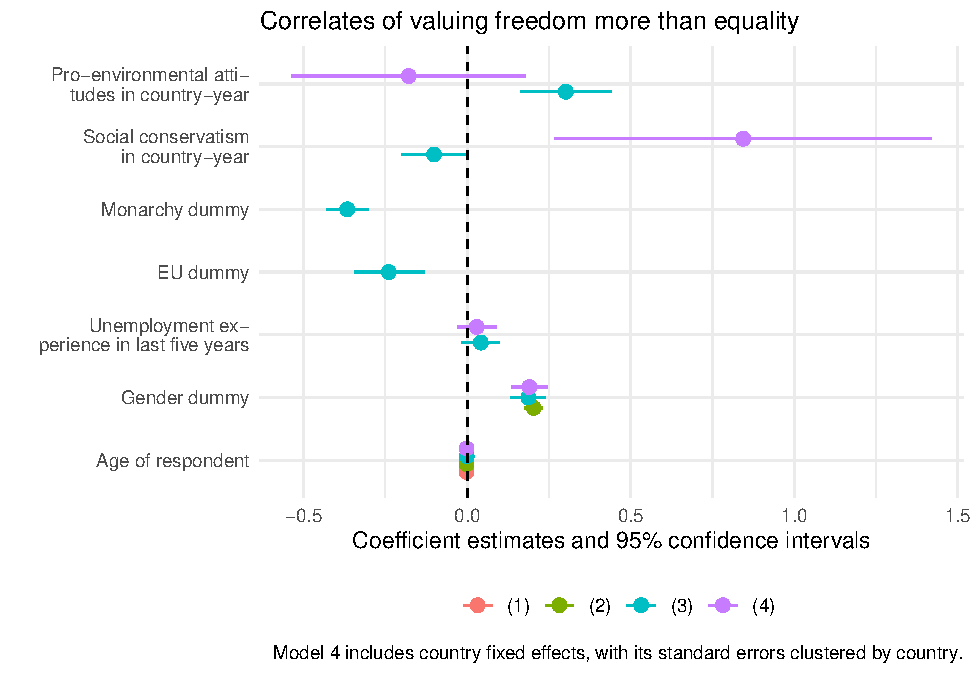
\includegraphics{AVCD-Assignment3-Edenhofer_files/figure-latex/free-better-correlates-1.pdf}

The coefficient plot implies four lessons:

\begin{itemize}
\item
  Gender is a statistically significant (at the 5\% level) predictor of
  valuing freedom more than equality across all models, with men being,
  on average, more likely to do so than females, holding all other
  included covariates constant. Substantively, the log odds are roughly
  20\% (\(100*(exp(0.18)-1)\)) higher for men than for females.
\item
  Age and unemployment experience do not significantly predict
  preferring freedom over equality.
\item
  On average, respondents residing in EU countries are, compared to
  their non-EU counterparts, significantly less likely to prefer freedom
  over equality, holding all other included covariates constant.
  Similarly, respondents residing in constitutional monarchies are less
  likely to express such a preference, relative to those living in
  republics. Substantively, the log odds are approximately 20\% lower
  (\(100*(exp(-0.239)-1)\)) for EU respondents, and 30\%
  (\(100*(exp(-0.367)-1)\)) lower for respondents in constitutional
  monarchies.
\item
  The inclusion of country fixed effects leads to a strongly positive
  association between overall social conservatism in a given year and a
  preference for freedom over equality, with the log odds increasing by
  roughly 130\% for a unit increase in social conservatism
  (\(100*(exp(0.84)-1)\)). By contrast, the coefficient estimate for
  pro-environmental attitudes becomes insignificant when including
  country fixed effects, suggesting that the original positive
  association is driven by (un)observed confounders.
\end{itemize}

To plot the predicted probabilities, I use the \texttt{ggpredict()}
function applied to a simple regression of \texttt{free\_better\_dummy}
on the interaction between \texttt{gndr\_dummy1} and
\texttt{uemp5yr\_factor}.

\begin{Shaded}
\begin{Highlighting}[]
\CommentTok{\# data }
\NormalTok{ess789\_mod }\OtherTok{\textless{}{-}}\NormalTok{ ess789\_mod }\SpecialCharTok{\%\textgreater{}\%}
  \FunctionTok{mutate}\NormalTok{(}\AttributeTok{gndr\_dummy1 =} \FunctionTok{factor}\NormalTok{(gndr\_dummy, }\AttributeTok{levels =} \FunctionTok{c}\NormalTok{(}\StringTok{"0"}\NormalTok{, }\StringTok{"1"}\NormalTok{), }
                             \AttributeTok{labels =} \FunctionTok{c}\NormalTok{(}\StringTok{"Female"}\NormalTok{, }\StringTok{"Male"}\NormalTok{)))}
\CommentTok{\# model }
\NormalTok{free\_better\_model5 }\OtherTok{\textless{}{-}} \FunctionTok{glm}\NormalTok{(free\_better\_dummy }\SpecialCharTok{\textasciitilde{}}\NormalTok{ gndr\_dummy1}\SpecialCharTok{*}\NormalTok{uemp5yr\_factor,}
                         \AttributeTok{family =} \FunctionTok{binomial}\NormalTok{(}\AttributeTok{link =} \StringTok{"logit"}\NormalTok{),}
                         \AttributeTok{data =}\NormalTok{ ess789\_mod)}
\CommentTok{\# plot }
\FunctionTok{plot}\NormalTok{(}\FunctionTok{ggpredict}\NormalTok{(free\_better\_model5, }\AttributeTok{terms =} \FunctionTok{c}\NormalTok{(}\StringTok{"gndr\_dummy1"}\NormalTok{, }\StringTok{"uemp5yr\_factor"}\NormalTok{)),}
     \AttributeTok{connect.lines =}\NormalTok{ T) }\SpecialCharTok{+}
  \FunctionTok{scale\_colour\_manual}\NormalTok{(}\StringTok{"Any period of unemployment or work seeking in the last five years?"}\NormalTok{,}
                        \AttributeTok{labels =} \FunctionTok{c}\NormalTok{(}\StringTok{"1"} \OtherTok{=} \StringTok{"Yes"}\NormalTok{,}
                                   \StringTok{"2"} \OtherTok{=} \StringTok{"No"}\NormalTok{),}
                        \AttributeTok{values =} \FunctionTok{c}\NormalTok{(}\StringTok{"1"} \OtherTok{=} \StringTok{"\#FFA500"}\NormalTok{,}
                                   \StringTok{"2"} \OtherTok{=} \StringTok{"\#0072B2"}\NormalTok{)) }\SpecialCharTok{+}
  \FunctionTok{labs}\NormalTok{(}\AttributeTok{x =} \StringTok{"Gender"}\NormalTok{, }\AttributeTok{y =} \StringTok{"Predicted probability"}\NormalTok{, }
       \AttributeTok{title =} \StringTok{"Predicted probabilities for valuing freedom more than equality"}\NormalTok{) }\SpecialCharTok{+}
  \FunctionTok{expand\_limits}\NormalTok{(}\AttributeTok{y =} \FunctionTok{c}\NormalTok{(}\FloatTok{0.2}\NormalTok{, }\FloatTok{0.3}\NormalTok{)) }\SpecialCharTok{+}
  \FunctionTok{theme}\NormalTok{(}\AttributeTok{legend.position =} \StringTok{"bottom"}\NormalTok{, }
        \AttributeTok{plot.title =} \FunctionTok{element\_text}\NormalTok{(}\AttributeTok{size =} \DecValTok{12}\NormalTok{))}
\end{Highlighting}
\end{Shaded}

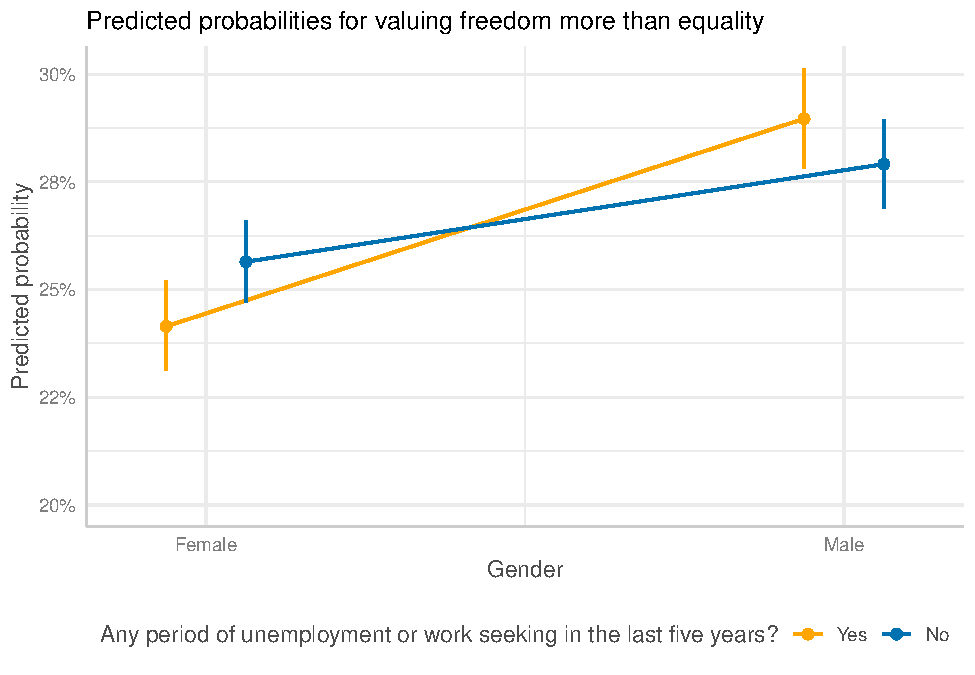
\includegraphics{AVCD-Assignment3-Edenhofer_files/figure-latex/predicted-probabilities-plot-1.pdf}

The vertical differences between the point estimates represent the
marginal effect of unemployment experience for men and women
respectively. For women, the marginal effect of having experienced
unemployment within the last five years is negative, while it is
positive for men. That is, men become significantly\footnote{The
  difference is significant at the 5\% level, which can be seen by
  running \texttt{summary(free\_better\_model5)}.} more likely to prefer
freedom over equality after having experienced unemployment, with the
reverse holding for women.

\hypertarget{section-3}{%
\subsection{1.4}\label{section-3}}

\textcolor{brown}{Estimate the model above using year-level fixed effects: What do the year-level fixed effects exactly do?, What are the variables that change? How? And why those in particular?}

By including year fixed effects, we restrict our attention to
cross-country variation within each ESS wave. Doing so allows us to
account for (confounding) factors, both observable and unobservable,
that vary over time and are constant across countries, such as common
economic shocks. Hence, I run:

\begin{Shaded}
\begin{Highlighting}[]
\NormalTok{free\_better\_model6 }\OtherTok{\textless{}{-}} \FunctionTok{bife}\NormalTok{(free\_better\_dummy }\SpecialCharTok{\textasciitilde{}}\NormalTok{ agea }\SpecialCharTok{+}\NormalTok{ gndr\_dummy }\SpecialCharTok{+}\NormalTok{ uemp5yr }\SpecialCharTok{+}\NormalTok{ eummbr\_factor }\SpecialCharTok{+}\NormalTok{ mnrchy\_factor }\SpecialCharTok{+}\NormalTok{ cons }\SpecialCharTok{+}\NormalTok{ env }\SpecialCharTok{|}\NormalTok{ year, }
           \AttributeTok{model =} \StringTok{"logit"}\NormalTok{, }\AttributeTok{data =}\NormalTok{ ess789\_mod)}
\CommentTok{\# coefficient plot, with previous models for comparison  }
\FunctionTok{modelplot}\NormalTok{(}\FunctionTok{list}\NormalTok{(free\_better\_model2, free\_better\_model3, }
\NormalTok{               free\_better\_model4, free\_better\_model6),}
          \AttributeTok{coef\_map =} \FunctionTok{c}\NormalTok{(}\StringTok{"agea"} \OtherTok{=} \StringTok{"Age of respondent"}\NormalTok{,}
                       \StringTok{"gndr\_dummy1"} \OtherTok{=} \StringTok{"Gender dummy"}\NormalTok{, }
                       \StringTok{"uemp5yr"} \OtherTok{=} \StringTok{"Unemployment ex{-}}\SpecialCharTok{\textbackslash{}n}\StringTok{perience in last five years"}\NormalTok{,}
                       \StringTok{"eummbr\_factor1"} \OtherTok{=} \StringTok{"EU dummy"}\NormalTok{, }
                       \StringTok{"mnrchy\_factor1"} \OtherTok{=} \StringTok{"Monarchy dummy"}\NormalTok{,}
                       \StringTok{"cons"} \OtherTok{=} \StringTok{"Social conservatism}\SpecialCharTok{\textbackslash{}n}\StringTok{in country{-}year"}\NormalTok{, }
                       \StringTok{"env"} \OtherTok{=} \StringTok{"Pro{-}environmental atti{-}}\SpecialCharTok{\textbackslash{}n}\StringTok{tudes in country{-}year"}\NormalTok{)) }\SpecialCharTok{+}
  \FunctionTok{geom\_vline}\NormalTok{(}\AttributeTok{xintercept =} \DecValTok{0}\NormalTok{, }\AttributeTok{linetype =} \StringTok{"dashed"}\NormalTok{) }\SpecialCharTok{+}
  \FunctionTok{labs}\NormalTok{(}\AttributeTok{title =} \StringTok{"Correlates of valuing freedom more than equality"}\NormalTok{, }
       \AttributeTok{caption =} \StringTok{"Model 3 includes country fixed effects; model 4 includes year fixed effects."}\NormalTok{) }\SpecialCharTok{+}
  \FunctionTok{theme}\NormalTok{(}\AttributeTok{legend.position =} \StringTok{"bottom"}\NormalTok{, }
        \AttributeTok{plot.title =} \FunctionTok{element\_text}\NormalTok{(}\AttributeTok{size =} \DecValTok{12}\NormalTok{))}
\end{Highlighting}
\end{Shaded}

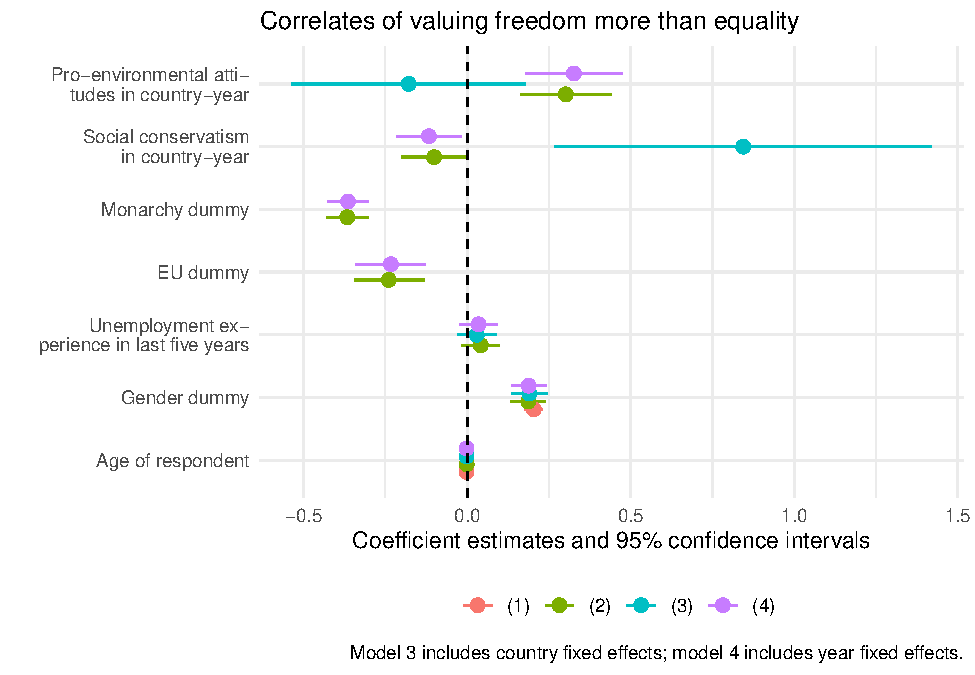
\includegraphics{AVCD-Assignment3-Edenhofer_files/figure-latex/year-fe-free-better-1.pdf}

We can see that the coefficient estimates yielded by the model with year
fixed effects are almost identical to the models we ran above, except
when comparing them to the coefficient estimates for \texttt{cons} and
\texttt{env} in the model with country fixed effects. For \texttt{env},
country fixed effects render the coefficient estimate insignificant, as
opposed to it being significantly positive. This suggests there are
time-invariant, country-specific factors that explain a fair amount of
the association between \texttt{env} and the preference for freedom over
equality. For \texttt{cons}, country fixed effects render the
coefficient estimate significantly positive, rather than significantly
negative, suggesting that wave-specific factors that are common across
countries have opposite effects to the time-invariant, country-specific
confounders country fixed effects control for.

\hypertarget{section-4}{%
\subsection{1.5}\label{section-4}}

\textcolor{brown}{If you were asked at which other level you would add fixed effects, what would you answer?}

Ideally, I would want to probe the robustness of the above results by
including year-wave fixed effects. In this way, we could control both
for country-specific, time-invariant (un)observable confounders (country
fixed effects), and for wave-specific, country-invariant (un)observable
confounders (wave fixed effects).

\hypertarget{exercise-2}{%
\section{Exercise 2}\label{exercise-2}}

\hypertarget{section-5}{%
\subsection{2.1}\label{section-5}}

\textcolor{brown}{Re-estimate the model above using year-level fixed effects. This time, however, use a different dependent variable: the level of country’s conservativism.}

I estimate four specifications with \texttt{cons} as the dependent
variable. I include fixed effects via the \texttt{feols()} function from
the \texttt{fixest} package, which is computationally more efficient
than the \texttt{plm()} function, and automatically clusters standard
errors at the level of the fixed effects (here the year level).

The justification of all covariates is, for the most part, analogous to
that offered in 1.3. The only exception is the inclusion of
\texttt{impfree\_recoded} and \texttt{ipeqopt\_recoded} in the final two
models. These variables are only contained in these models because they
may be strongly multi-collinear with other variables, thereby
potentially inflating the standard errors of the coefficient estimates
and increasing the risk of type II errors. To mitigate this risk, I
estimate specifications with and without these two variables.

\begin{Shaded}
\begin{Highlighting}[]
\NormalTok{socio\_cons\_year\_fe1 }\OtherTok{\textless{}{-}} \FunctionTok{feols}\NormalTok{(cons }\SpecialCharTok{\textasciitilde{}}\NormalTok{ gndr\_dummy }\SpecialCharTok{+}\NormalTok{ agea }\SpecialCharTok{+}\NormalTok{ uemp5yr\_factor }\SpecialCharTok{|}\NormalTok{ year, }\AttributeTok{data =}\NormalTok{ ess789\_mod)}
\NormalTok{socio\_cons\_year\_fe2 }\OtherTok{\textless{}{-}} \FunctionTok{feols}\NormalTok{(cons }\SpecialCharTok{\textasciitilde{}}\NormalTok{ gndr\_dummy }\SpecialCharTok{+}\NormalTok{ agea }\SpecialCharTok{+}\NormalTok{ uemp5yr\_factor }\SpecialCharTok{+} 
\NormalTok{                              eummbr\_factor }\SpecialCharTok{+}\NormalTok{ mnrchy\_factor }\SpecialCharTok{|}\NormalTok{ year, }\AttributeTok{data =}\NormalTok{ ess789\_mod)}
\NormalTok{socio\_cons\_year\_fe3 }\OtherTok{\textless{}{-}} \FunctionTok{feols}\NormalTok{(cons }\SpecialCharTok{\textasciitilde{}}\NormalTok{ gndr\_dummy }\SpecialCharTok{+}\NormalTok{ agea }\SpecialCharTok{+}\NormalTok{ uemp5yr\_factor }\SpecialCharTok{+} 
\NormalTok{                              eummbr\_factor }\SpecialCharTok{+}\NormalTok{ mnrchy\_factor }\SpecialCharTok{+}\NormalTok{ impfree\_recoded }\SpecialCharTok{|}\NormalTok{ year, }\AttributeTok{data =}\NormalTok{ ess789\_mod)}
\NormalTok{socio\_cons\_year\_fe4 }\OtherTok{\textless{}{-}} \FunctionTok{feols}\NormalTok{(cons }\SpecialCharTok{\textasciitilde{}}\NormalTok{ gndr\_dummy }\SpecialCharTok{+}\NormalTok{ agea }\SpecialCharTok{+}\NormalTok{ uemp5yr\_factor }\SpecialCharTok{+} 
\NormalTok{                              eummbr\_factor }\SpecialCharTok{+}\NormalTok{ mnrchy\_factor }\SpecialCharTok{+}\NormalTok{ impfree\_recoded }\SpecialCharTok{+}\NormalTok{ ipeqopt\_recoded }\SpecialCharTok{|}\NormalTok{ year, }\AttributeTok{data =}\NormalTok{ ess789\_mod)}

\CommentTok{\# coefficient plot }
\FunctionTok{modelplot}\NormalTok{(}\FunctionTok{list}\NormalTok{(socio\_cons\_year\_fe1, socio\_cons\_year\_fe2, }
\NormalTok{                socio\_cons\_year\_fe3, socio\_cons\_year\_fe4),}
          \AttributeTok{coef\_map =} \FunctionTok{c}\NormalTok{(}\StringTok{"ipeqopt\_recoded"} \OtherTok{=} \StringTok{"Equal treatment/opportunity"}\NormalTok{, }
                       \StringTok{"impfree\_recoded"} \OtherTok{=} \StringTok{"Importance of freedom"}\NormalTok{, }
                       \StringTok{"mnrchy\_factor1"} \OtherTok{=} \StringTok{"Monarchy dummy"}\NormalTok{, }
                       \StringTok{"eummbr\_factor1"} \OtherTok{=} \StringTok{"EU dummy"}\NormalTok{, }
                       \StringTok{"uemp5yr\_factor2"} \OtherTok{=} \StringTok{"Unemployment dummy"}\NormalTok{, }
                       \StringTok{"agea"} \OtherTok{=} \StringTok{"Age"}\NormalTok{, }
                       \StringTok{"gndr\_dummy1"} \OtherTok{=} \StringTok{"Gender dummy"}\NormalTok{)) }\SpecialCharTok{+}
  \FunctionTok{geom\_vline}\NormalTok{(}\AttributeTok{xintercept =} \DecValTok{0}\NormalTok{, }\AttributeTok{linetype =} \StringTok{"dashed"}\NormalTok{) }\SpecialCharTok{+}
  \FunctionTok{labs}\NormalTok{(}\AttributeTok{title =} \StringTok{"Correlates of social conservatism at the country{-}year level"}\NormalTok{, }
       \AttributeTok{caption =} \StringTok{"All models include year fixed effects, with standard errors clustered by year."}\NormalTok{) }\SpecialCharTok{+}
  \FunctionTok{theme}\NormalTok{(}\AttributeTok{legend.position =} \StringTok{"bottom"}\NormalTok{, }
        \AttributeTok{plot.title =} \FunctionTok{element\_text}\NormalTok{(}\AttributeTok{size =} \DecValTok{12}\NormalTok{))}
\end{Highlighting}
\end{Shaded}

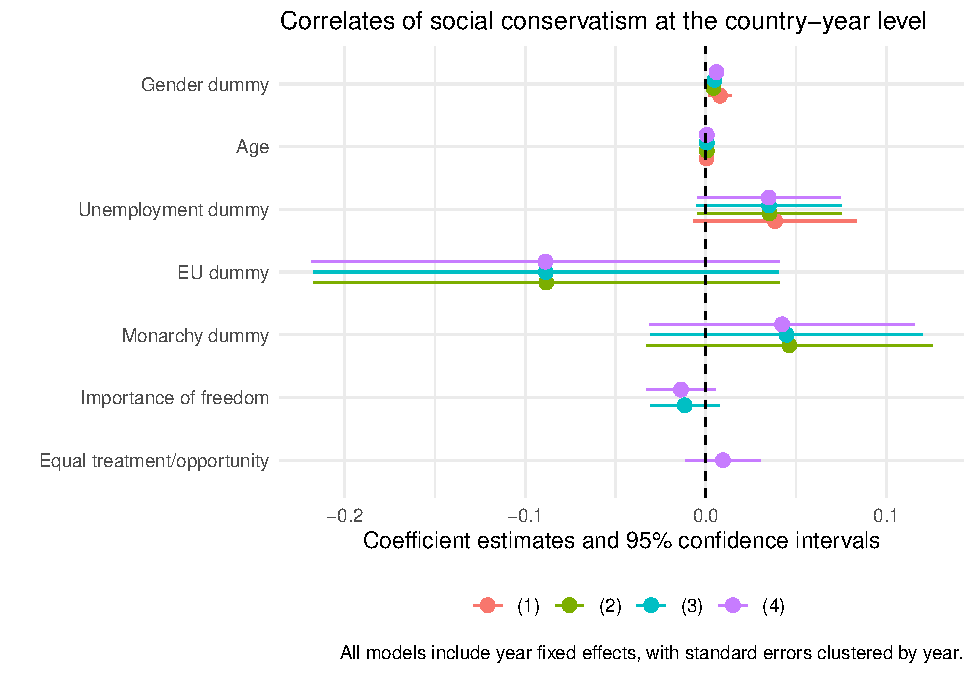
\includegraphics{AVCD-Assignment3-Edenhofer_files/figure-latex/socio-cons-year-fe-1.pdf}

The coefficient plot shows that only gender is a significant predictor
of social conservatism once year fixed effects are taken into account,
with males being slightly more likely than females to be socially
conservative.

\hypertarget{section-6}{%
\subsection{2.2}\label{section-6}}

\textcolor{brown}{Re-estimate the model above using country-level fixed effects. (Hint: what class is the variable for country? Is it the most appropriate?) Plot the coefficients: What does it change with respect with the model with year fixed effects? Why?}

The logic of the four models below is analogous to the previous
exercise, save for country fixed effects replacing year fixed effects.
As discussed above, country fixed effects net out all (un)observed,
country-specific factors that are constant over time. To illustrate
this, I have included \texttt{eummbr\_factor} and
\texttt{mnrchy\_factor}, which are constant within countries over time.
R automatically drops these variables since they are already accounted
for via the country fixed effects, which is why they are not represented
in the coefficient plot below.

\begin{Shaded}
\begin{Highlighting}[]
\CommentTok{\# turn country into factor }
\NormalTok{ess789\_mod }\OtherTok{\textless{}{-}}\NormalTok{ ess789\_mod }\SpecialCharTok{\%\textgreater{}\%}
  \FunctionTok{mutate}\NormalTok{(}\AttributeTok{cntry\_factor =} \FunctionTok{factor}\NormalTok{(cntry))}

\CommentTok{\# models}
\NormalTok{socio\_cons\_cntry\_fe1 }\OtherTok{\textless{}{-}} \FunctionTok{feols}\NormalTok{(cons }\SpecialCharTok{\textasciitilde{}}\NormalTok{ gndr\_dummy }\SpecialCharTok{+}\NormalTok{ agea }\SpecialCharTok{+}\NormalTok{ uemp5yr\_factor }\SpecialCharTok{|}\NormalTok{ cntry\_factor, }
                              \AttributeTok{data =}\NormalTok{ ess789\_mod)}
\NormalTok{socio\_cons\_cntry\_fe2 }\OtherTok{\textless{}{-}} \FunctionTok{feols}\NormalTok{(cons }\SpecialCharTok{\textasciitilde{}}\NormalTok{ gndr\_dummy }\SpecialCharTok{+}\NormalTok{ agea }\SpecialCharTok{+}\NormalTok{ uemp5yr\_factor }\SpecialCharTok{+} 
\NormalTok{                              eummbr\_factor }\SpecialCharTok{+}\NormalTok{ mnrchy\_factor }\SpecialCharTok{|}\NormalTok{ cntry\_factor, }
                              \AttributeTok{data =}\NormalTok{ ess789\_mod)}
\NormalTok{socio\_cons\_cntry\_fe3 }\OtherTok{\textless{}{-}} \FunctionTok{feols}\NormalTok{(cons }\SpecialCharTok{\textasciitilde{}}\NormalTok{ gndr\_dummy }\SpecialCharTok{+}\NormalTok{ agea }\SpecialCharTok{+}\NormalTok{ uemp5yr\_factor }\SpecialCharTok{+} 
\NormalTok{                              eummbr\_factor }\SpecialCharTok{+}\NormalTok{ mnrchy\_factor }\SpecialCharTok{+}\NormalTok{ impfree\_recoded }\SpecialCharTok{|}\NormalTok{ cntry\_factor, }
                              \AttributeTok{data =}\NormalTok{ ess789\_mod)}
\NormalTok{socio\_cons\_cntry\_fe4 }\OtherTok{\textless{}{-}} \FunctionTok{feols}\NormalTok{(cons }\SpecialCharTok{\textasciitilde{}}\NormalTok{ gndr\_dummy }\SpecialCharTok{+}\NormalTok{ agea }\SpecialCharTok{+}\NormalTok{ uemp5yr\_factor }\SpecialCharTok{+} 
\NormalTok{                              eummbr\_factor }\SpecialCharTok{+}\NormalTok{ mnrchy\_factor }\SpecialCharTok{+}\NormalTok{ impfree\_recoded }\SpecialCharTok{+}\NormalTok{ ipeqopt\_recoded }\SpecialCharTok{|}\NormalTok{ cntry\_factor, }
                              \AttributeTok{data =}\NormalTok{ ess789\_mod)}

\CommentTok{\# models }
\FunctionTok{modelplot}\NormalTok{(}\FunctionTok{list}\NormalTok{(socio\_cons\_cntry\_fe1, socio\_cons\_cntry\_fe2, }
\NormalTok{               socio\_cons\_cntry\_fe3, socio\_cons\_cntry\_fe4),}
          \AttributeTok{coef\_map =} \FunctionTok{c}\NormalTok{(}\StringTok{"ipeqopt\_recoded"} \OtherTok{=} \StringTok{"Equal treatment/opportunity"}\NormalTok{, }
                       \StringTok{"impfree\_recoded"} \OtherTok{=} \StringTok{"Importance of freedom"}\NormalTok{, }
                       \StringTok{"mnrchy\_factor1"} \OtherTok{=} \StringTok{"Monarchy dummy"}\NormalTok{, }
                       \StringTok{"eummbr\_factor1"} \OtherTok{=} \StringTok{"EU dummy"}\NormalTok{, }
                       \StringTok{"uemp5yr\_factor2"} \OtherTok{=} \StringTok{"Unemployment dummy"}\NormalTok{, }
                       \StringTok{"agea"} \OtherTok{=} \StringTok{"Age"}\NormalTok{, }
                       \StringTok{"gndr\_dummy1"} \OtherTok{=} \StringTok{"Gender dummy"}\NormalTok{)) }\SpecialCharTok{+}
  \FunctionTok{geom\_vline}\NormalTok{(}\AttributeTok{xintercept =} \DecValTok{0}\NormalTok{, }\AttributeTok{linetype =} \StringTok{"dashed"}\NormalTok{) }\SpecialCharTok{+}
  \FunctionTok{expand\_limits}\NormalTok{(}\AttributeTok{x =} \SpecialCharTok{{-}}\FloatTok{0.005}\NormalTok{) }\SpecialCharTok{+}
  \FunctionTok{labs}\NormalTok{(}\AttributeTok{title =} \StringTok{"Correlates of social conservatism at the country{-}year level"}\NormalTok{, }
       \AttributeTok{caption =} \StringTok{"All models include country fixed effects, with standard errors clustered by country."}\NormalTok{) }\SpecialCharTok{+}
  \FunctionTok{theme}\NormalTok{(}\AttributeTok{legend.position =} \StringTok{"bottom"}\NormalTok{, }
        \AttributeTok{plot.title =} \FunctionTok{element\_text}\NormalTok{(}\AttributeTok{size =} \DecValTok{12}\NormalTok{))}
\end{Highlighting}
\end{Shaded}

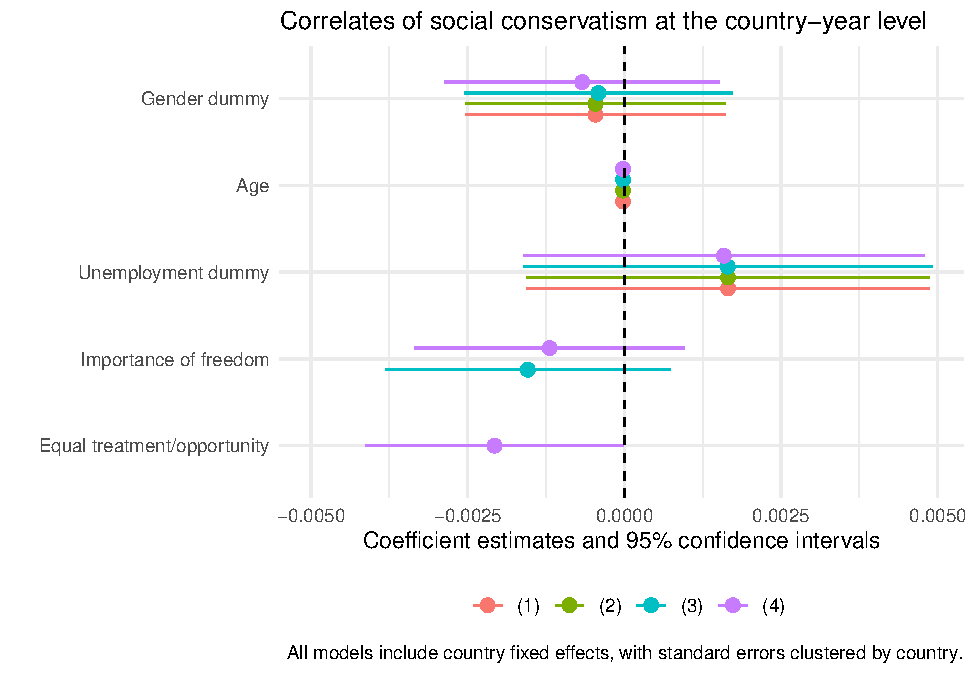
\includegraphics{AVCD-Assignment3-Edenhofer_files/figure-latex/socio-cons-cntry-fe-1.pdf}

The coefficient plot demonstrates that, within a given country,
respondents' belief in equality is significantly and negatively
associated with social conservatism in that country in a given year,
while all other covariates are insignificant.

\hypertarget{section-7}{%
\subsection{2.3}\label{section-7}}

\textcolor{brown}{Random Effects: estimate the model using random effects for years and country}

To estimate the desired models, I estimate four specifications, where
the logic underpinning the choice of covariates is analogous to the
previous exercises. The only difference is that I use the
\texttt{lmer()} to include random effects for years and country.

\begin{Shaded}
\begin{Highlighting}[]
\NormalTok{socio\_cons\_re1 }\OtherTok{\textless{}{-}} \FunctionTok{lmer}\NormalTok{(cons }\SpecialCharTok{\textasciitilde{}}\NormalTok{ gndr\_dummy }\SpecialCharTok{+}\NormalTok{ agea }\SpecialCharTok{+}\NormalTok{ uemp5yr\_factor }\SpecialCharTok{+}\NormalTok{ (}\DecValTok{1} \SpecialCharTok{+}\NormalTok{ essround }\SpecialCharTok{|}\NormalTok{ cntry),}
                       \AttributeTok{data =}\NormalTok{ ess789\_mod,}
                       \AttributeTok{control =} \FunctionTok{lmerControl}\NormalTok{(}\AttributeTok{optimizer =} \StringTok{"nloptwrap"}\NormalTok{))}
\NormalTok{socio\_cons\_re2 }\OtherTok{\textless{}{-}} \FunctionTok{lmer}\NormalTok{(cons }\SpecialCharTok{\textasciitilde{}}\NormalTok{ gndr\_dummy }\SpecialCharTok{+}\NormalTok{ agea }\SpecialCharTok{+}\NormalTok{ uemp5yr\_factor }\SpecialCharTok{+}\NormalTok{ eummbr\_factor }\SpecialCharTok{+}\NormalTok{ mnrchy\_factor }\SpecialCharTok{+}
\NormalTok{                         (}\DecValTok{1} \SpecialCharTok{+}\NormalTok{ essround }\SpecialCharTok{|}\NormalTok{ cntry), }
                       \AttributeTok{control =} \FunctionTok{lmerControl}\NormalTok{(}\AttributeTok{optimizer =} \StringTok{"nloptwrap"}\NormalTok{),}
                       \AttributeTok{data =}\NormalTok{ ess789\_mod)}
\NormalTok{socio\_cons\_re3 }\OtherTok{\textless{}{-}} \FunctionTok{lmer}\NormalTok{(cons }\SpecialCharTok{\textasciitilde{}}\NormalTok{ gndr\_dummy }\SpecialCharTok{+}\NormalTok{ agea }\SpecialCharTok{+}\NormalTok{ uemp5yr\_factor }\SpecialCharTok{+}\NormalTok{ eummbr\_factor }\SpecialCharTok{+}\NormalTok{ mnrchy\_factor }\SpecialCharTok{+} 
\NormalTok{                        impfree\_recoded }\SpecialCharTok{+}\NormalTok{ ipeqopt\_recoded }\SpecialCharTok{+}\NormalTok{ (}\DecValTok{1} \SpecialCharTok{+}\NormalTok{ essround }\SpecialCharTok{|}\NormalTok{ cntry), }
                       \AttributeTok{control =} \FunctionTok{lmerControl}\NormalTok{(}\AttributeTok{optimizer =} \StringTok{"nloptwrap"}\NormalTok{),}
                       \AttributeTok{data =}\NormalTok{ ess789\_mod)}
\CommentTok{\# modelsummary }
\FunctionTok{modelplot}\NormalTok{(}\FunctionTok{list}\NormalTok{(socio\_cons\_re1, socio\_cons\_re2, socio\_cons\_re3),}
          \AttributeTok{coef\_map =} \FunctionTok{c}\NormalTok{(}\StringTok{"ipeqopt\_recoded"} \OtherTok{=} \StringTok{"Equal treatment/opportunity"}\NormalTok{, }
                       \StringTok{"impfree\_recoded"} \OtherTok{=} \StringTok{"Importance of freedom"}\NormalTok{, }
                       \StringTok{"mnrchy\_factor1"} \OtherTok{=} \StringTok{"Monarchy dummy"}\NormalTok{, }
                       \StringTok{"eummbr\_factor1"} \OtherTok{=} \StringTok{"EU dummy"}\NormalTok{, }
                       \StringTok{"uemp5yr\_factor2"} \OtherTok{=} \StringTok{"Unemployment dummy"}\NormalTok{, }
                       \StringTok{"agea"} \OtherTok{=} \StringTok{"Age"}\NormalTok{, }
                       \StringTok{"gndr\_dummy1"} \OtherTok{=} \StringTok{"Gender dummy"}\NormalTok{)) }\SpecialCharTok{+}
  \FunctionTok{geom\_vline}\NormalTok{(}\AttributeTok{xintercept =} \DecValTok{0}\NormalTok{, }\AttributeTok{linetype =} \StringTok{"dashed"}\NormalTok{) }\SpecialCharTok{+}
  \FunctionTok{expand\_limits}\NormalTok{(}\AttributeTok{x =} \FunctionTok{c}\NormalTok{(}\SpecialCharTok{{-}}\FloatTok{0.6}\NormalTok{, }\FloatTok{0.4}\NormalTok{)) }\SpecialCharTok{+}
  \FunctionTok{labs}\NormalTok{(}\AttributeTok{title =} \StringTok{"Correlates of social conservatism at the country{-}year level"}\NormalTok{, }
       \AttributeTok{caption =} \StringTok{"All models include random effects for countries and years."}\NormalTok{) }\SpecialCharTok{+}
  \FunctionTok{theme}\NormalTok{(}\AttributeTok{legend.position =} \StringTok{"bottom"}\NormalTok{, }
        \AttributeTok{plot.title =} \FunctionTok{element\_text}\NormalTok{(}\AttributeTok{size =} \DecValTok{12}\NormalTok{))}
\end{Highlighting}
\end{Shaded}

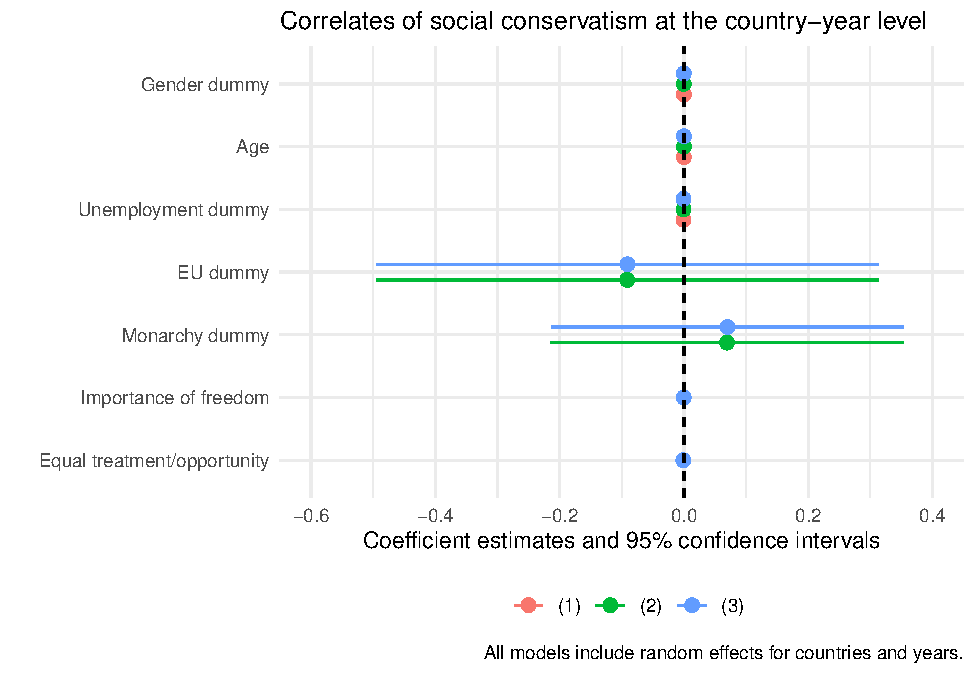
\includegraphics{AVCD-Assignment3-Edenhofer_files/figure-latex/socio-cons-cntry-year-re-1.pdf}

Once we include random effects for countries and years, none of the
predictors is statistically significant.

\hypertarget{section-8}{%
\subsection{2.4}\label{section-8}}

\textcolor{brown}{What do fixed effects account for? Specify: for years and countries/geographic regions, What do random effects account for?, Following Schimdt-Catran and Fairbrother, illustrate the structure of fixed effects.}

Year fixed effects\footnote{Mummolo and Peterson
  (\protect\hyperlink{ref-mummolo2018improving}{2018}) make a number of
  important points about the proper use of fixed effects. To improve the
  interpretation of fixed effects, the authors recommend: ``Identify a
  plausible counterfactual shift in X given the data: Generate a
  histogram of the within-unit ranges of the treatment to get a sense of
  the relevant shifts in X that occur in the data. Compute the standard
  deviation of the transformed (residualized) independent variable,
  which can be thought of as a typical shift in the portion of the
  independent variable that is being used during the fixed effects
  estimation. Multiply the estimated coefficient of interest by the
  revised standard deviation of the independent variable to assess
  substantive importance. Note for readers what share of observations do
  not exhibit any variation within units to help characterize the
  generalizability of the result. Alternatively, if describing the
  effect of a one-unit shift, or any other quantity, note the ratio of
  this shift in X to the within-unit standard deviation, as well as its
  location on the recommended histogram, to gauge how typically a shift
  of this size occurs within units.''
  (\protect\hyperlink{ref-mummolo2018improving}{Mummolo and Peterson
  2018, 833--34})}, applied to repeated cross-sectional or panel data,
control for \emph{all} (un)observable confounders, viz.~variables that
affect both the explanatory and dependent variables of interest, that
are constant across units (e.g.~individual respondents, regions,
countries, etc.), while varying over time. Put more intuitively, year
fixed effects allow us to control for ``shocks'' that vary over time,
but are common to all units. Regional fixed effects, by contrast,
control for all (un)observable confounders that are constant over time,
while varying across countries. That is, unit fixed effects exploit only
within-unit variation over time. When our regions are countries, country
fixed effects can, for instance, net out cultural confounders, which
tend to be constant over time. Following Schmidt-Catran and Fairbrother
(\protect\hyperlink{ref-schmidt2016random}{2016}), we can represent the
underlying data structure for these two types of fixed effects as
follows:

\begin{Shaded}
\begin{Highlighting}[]
\CommentTok{\# packages }
\FunctionTok{library}\NormalTok{(DiagrammeRsvg)}
\FunctionTok{library}\NormalTok{(magrittr)}
\FunctionTok{library}\NormalTok{(svglite)}
\FunctionTok{library}\NormalTok{(rsvg)}
\FunctionTok{library}\NormalTok{(png)}
\FunctionTok{library}\NormalTok{(ggdag)}
\FunctionTok{library}\NormalTok{(DiagrammeR)}
\FunctionTok{library}\NormalTok{(tidyverse)}

\CommentTok{\# graphs }
\NormalTok{g1 }\OtherTok{\textless{}{-}} \FunctionTok{grViz}\NormalTok{(}\StringTok{"}
\StringTok{    digraph causal \{}
\StringTok{    graph [ranksep = 0.2, fontsize = 5, rankdir = TB]}
\StringTok{      \# Nodes}
\StringTok{      node [shape = square, style = filled, fillcolor = dimgray, width = 2.2, fixedsize=true, fontsize = 16, fontname = \textquotesingle{}Gudea\textquotesingle{}]}
\StringTok{      A [label = \textquotesingle{}Fixed effects (FEs)\textquotesingle{}]}
\StringTok{      node [shape = square, style = filled, fillcolor = darkgreen, width = 2.2, fixedsize=true, fontsize = 16, fontname = \textquotesingle{}Gudea\textquotesingle{}]}
\StringTok{      B [label = \textquotesingle{}Regional FEs}\SpecialCharTok{\textbackslash{}n}\StringTok{(e.g. country, local}\SpecialCharTok{\textbackslash{}n}\StringTok{authority,}\SpecialCharTok{\textbackslash{}n}\StringTok{federal state)\textquotesingle{}]}
\StringTok{      C [label = \textquotesingle{}Year FEs\textquotesingle{}]}
\StringTok{      node [shape = circle, style = filled, fillcolor = \textquotesingle{}\#4576B7\textquotesingle{}, width = 2.2, fixedsize=true, fontsize = 16, fontname = \textquotesingle{}Gudea\textquotesingle{}]}
\StringTok{      E [label = \textquotesingle{}Region\textquotesingle{}]}
\StringTok{      F [label = \textquotesingle{}Year\textquotesingle{}]}
\StringTok{      node [shape = circle, style = filled, fillcolor = \textquotesingle{}\#FF9800\textquotesingle{}, width = 2.2, fixedsize=true, fontsize = 16, fontname = \textquotesingle{}Gudea\textquotesingle{}]}
\StringTok{      E1 [label = \textquotesingle{}Individual 1}\SpecialCharTok{\textbackslash{}n}\StringTok{in year 1\textquotesingle{}]}
\StringTok{      E2 [label = \textquotesingle{}Individual 1}\SpecialCharTok{\textbackslash{}n}\StringTok{in year 2\textquotesingle{}]}
\StringTok{      E3 [label = \textquotesingle{}Individual 1}\SpecialCharTok{\textbackslash{}n}\StringTok{in year T\textquotesingle{}]}
\StringTok{      E4 [label = \textquotesingle{}...\textquotesingle{}]}
\StringTok{      E5 [label = \textquotesingle{}Individual N}\SpecialCharTok{\textbackslash{}n}\StringTok{in year T\textquotesingle{}]}
\StringTok{      F1 [label = \textquotesingle{}Individual 1}\SpecialCharTok{\textbackslash{}n}\StringTok{in region 1\textquotesingle{}]}
\StringTok{      F2 [label = \textquotesingle{}Individual 2}\SpecialCharTok{\textbackslash{}n}\StringTok{in region 1\textquotesingle{}]}
\StringTok{      F3 [label = \textquotesingle{}Individual N}\SpecialCharTok{\textbackslash{}n}\StringTok{in region 1\textquotesingle{}]}
\StringTok{      F4 [label = \textquotesingle{}...\textquotesingle{}]}
\StringTok{      F5 [label = \textquotesingle{}Individual N}\SpecialCharTok{\textbackslash{}n}\StringTok{in region X\textquotesingle{}]}
\StringTok{      \# Edges}
\StringTok{       edge [color = \textquotesingle{}\#666666\textquotesingle{}, minlen = 4, arrowhead = vee, penwidth = 2.5]}
\StringTok{      A{-}\textgreater{}\{B C\}}
\StringTok{      B{-}\textgreater{}E}
\StringTok{      C{-}\textgreater{}F}
\StringTok{      E{-}\textgreater{}\{E1 E2 E3 E4 E5\}}
\StringTok{      F{-}\textgreater{}\{F1 F2 F3 F4 F5\}}
\StringTok{   \{rank = same; E; F\}}
\StringTok{    \}"}\NormalTok{)}

\CommentTok{\# save as image }
\NormalTok{g1 }\SpecialCharTok{\%\textgreater{}\%}
  \FunctionTok{export\_svg}\NormalTok{() }\SpecialCharTok{\%\textgreater{}\%}
  \FunctionTok{charToRaw}\NormalTok{() }\SpecialCharTok{\%\textgreater{}\%}
  \FunctionTok{rsvg\_png}\NormalTok{(}\StringTok{"fe\_overview.png"}\NormalTok{)}

\CommentTok{\# include image }
\FunctionTok{include\_graphics}\NormalTok{(}\AttributeTok{path =} \StringTok{"fe\_overview.png"}\NormalTok{)}
\end{Highlighting}
\end{Shaded}

\begin{figure}
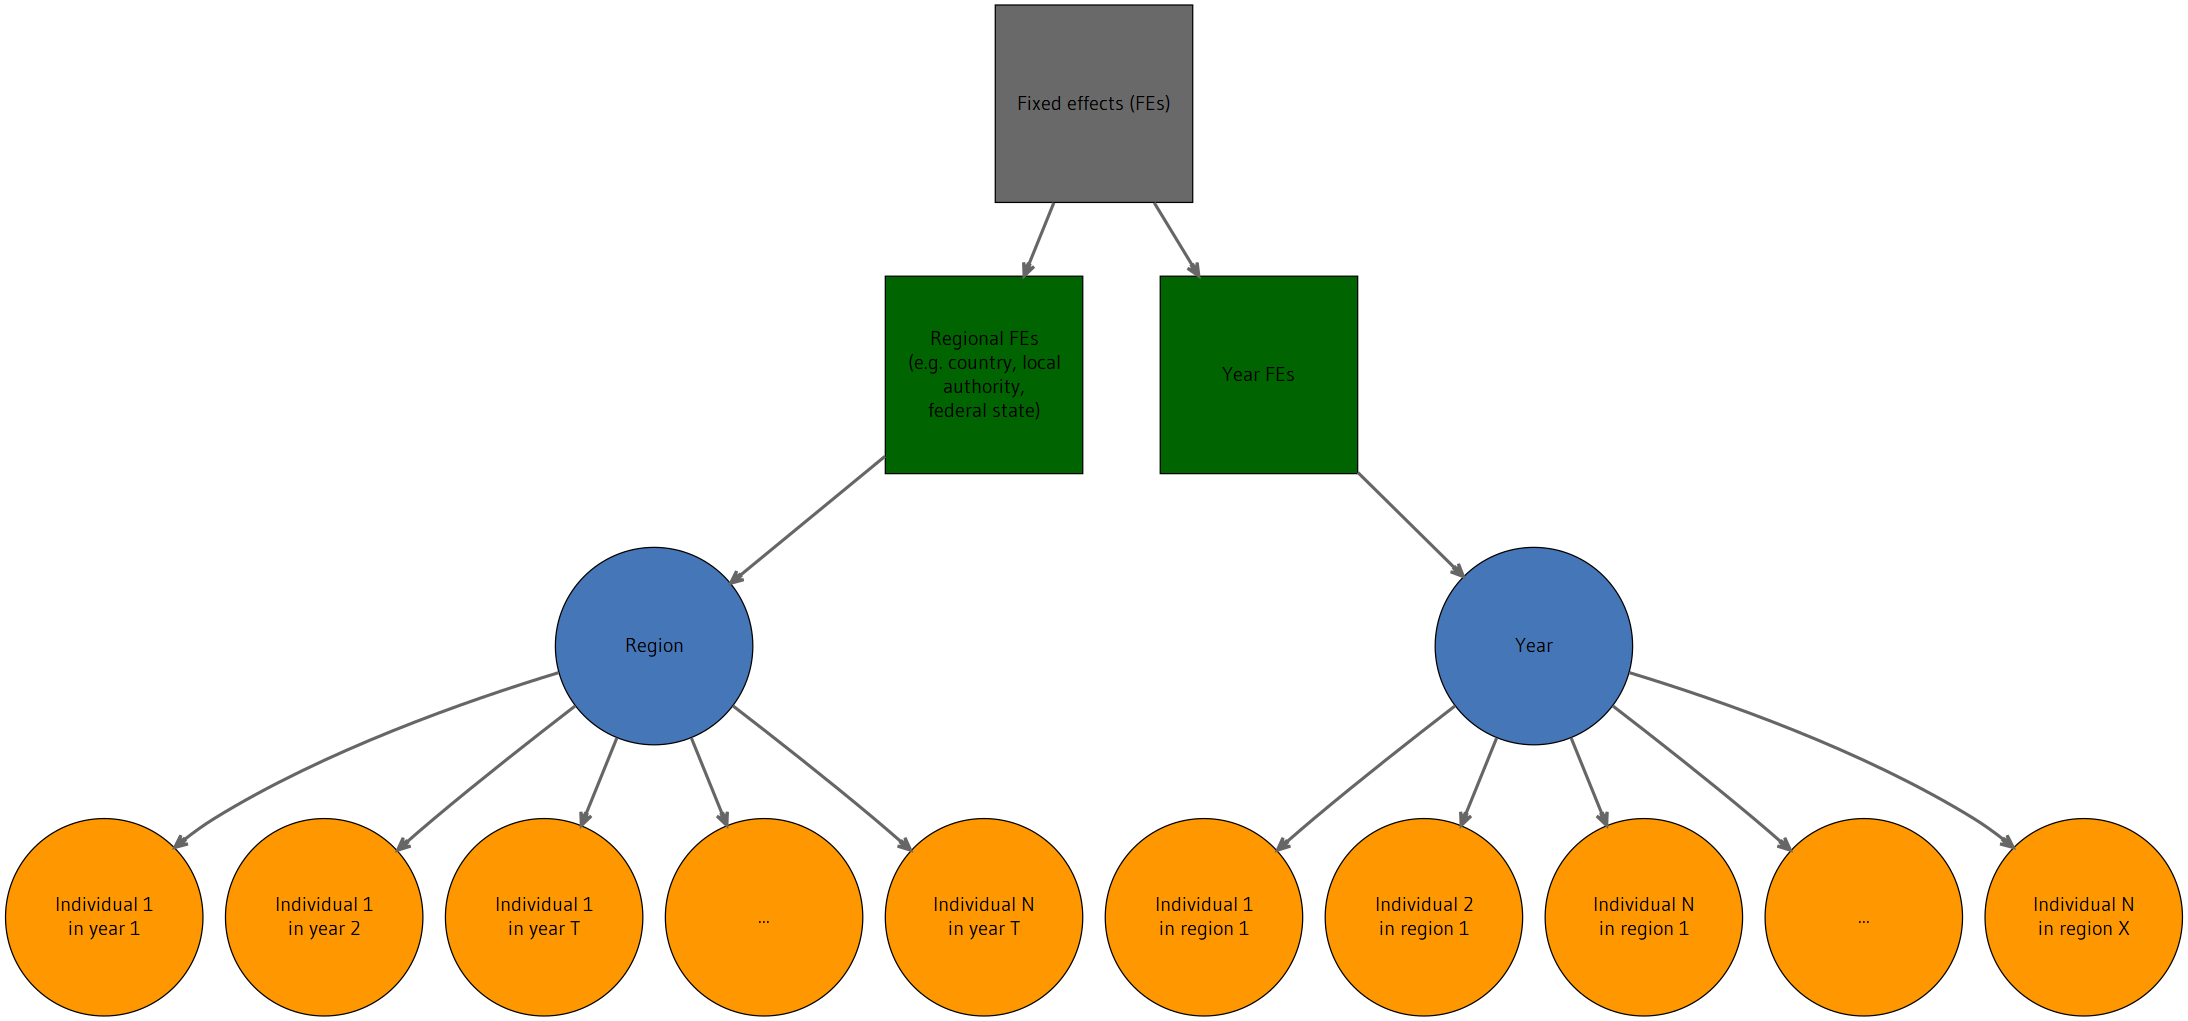
\includegraphics[width=1\linewidth]{fe_overview} \caption{Overview of data structures for different types of fixed effects}\label{fig:fe-representation-data-structure}
\end{figure}

Random effects, by contrast, account for all factors that (i) affect the
outcome, and (ii) vary randomly across individuals or groups, provided
they are not correlated with (un)observed determinants of the outcome
that the error term captures.

\FloatBarrier

\hypertarget{references}{%
\section*{References}\label{references}}
\addcontentsline{toc}{section}{References}

\hypertarget{refs}{}
\begin{CSLReferences}{1}{0}
\leavevmode\vadjust pre{\hypertarget{ref-anduiza2022sexism}{}}%
Anduiza, Eva, and Guillem Rico. 2022. {``Sexism and the Far-Right Vote:
The Individual Dynamics of Gender Backlash.''} \emph{American Journal of
Political Science}.

\leavevmode\vadjust pre{\hypertarget{ref-inglehart2010changing}{}}%
Inglehart, Ronald, and Christian Welzel. 2010. {``Changing Mass
Priorities: The Link Between Modernization and Democracy.''}
\emph{Perspectives on Politics} 8 (2): 551--67.

\leavevmode\vadjust pre{\hypertarget{ref-mummolo2018improving}{}}%
Mummolo, Jonathan, and Erik Peterson. 2018. {``Improving the
Interpretation of Fixed Effects Regression Results.''} \emph{Political
Science Research and Methods} 6 (4): 829--35.

\leavevmode\vadjust pre{\hypertarget{ref-oshri2022risk}{}}%
Oshri, Odelia, Liran Harsgor, Reut Itzkovitch-Malka, and Or Tuttnauer.
2022. {``Risk Aversion and the Gender Gap in the Vote for Populist
Radical Right Parties.''} \emph{American Journal of Political Science}.

\leavevmode\vadjust pre{\hypertarget{ref-schmidt2016random}{}}%
Schmidt-Catran, Alexander W, and Malcolm Fairbrother. 2016. {``The
Random Effects in Multilevel Models: Getting Them Wrong and Getting Them
Right.''} \emph{European Sociological Review} 32 (1): 23--38.

\end{CSLReferences}

\end{document}
